\documentclass[../main.tex]{subfiles}
\begin{document}

\ifSubfilesClassLoaded{
	\mainmatter
	\setcounter{chapter}{1}
}{}

\chapter{SeaQuest Experiment}
\label{ch:seaquest}

\section{Introduction}
SeaQuest is a fixed-target experiment utilizing the \SI{120}{\GeV} proton beam
from the Fermilab Main Injector. Details of the SeaQuest spectrometer can be
found in Ref.~\cite{aidala2019}. A schematics of the spectrometer is shown in
\cref{fig:spectrometer}. The target system consists of seven
interchangeable targets, including a flask with liquid hydrogen, a flask with
liquid deuterium,an empty flask (vacuum), solid carbon, iron, and tungsten
targets as well as a space with no target (air). The targets are interchanged
periodically to reduce systematic uncertainties in the measured cross section
ratios for different targets.

The spectrometer consists of two magnets and four tracking stations. FMag,
placed \SI{104}{\cm} downstream the target, is a \SI{5}{\m} solid iron magnet
that acts as the beam dump as well as a focusing magnet. It is then followed by
the first tracking stations. Stations 1, 2 and 3 each consists of plastic
scintillator hodoscopes and drift chambers. An open air dipole magnet (KMag) is
placed between station 1 and station 2. The vertical magnetic field from both
magnets bends the muons horizontally, allowing the measurement of the momentum
of the muons. Downstream of station 3, there is a 1 m iron wall acting as a
hadron absorber. Station 4 is located behind the hadron absorber and acts as a
muon identifier. Station 4 consists of a hodoscope array and 4 layers of
proportional tube planes. Tracks that pass through the hadron absorber and
produce hits on station 4 are assumed to be from muons.
\pdfmargincomment{Should there be a dedicated section on the spectrometer?
	how much detail of the spectrometer is need?
}

\begin{figure}[htbp!]
	\centering
	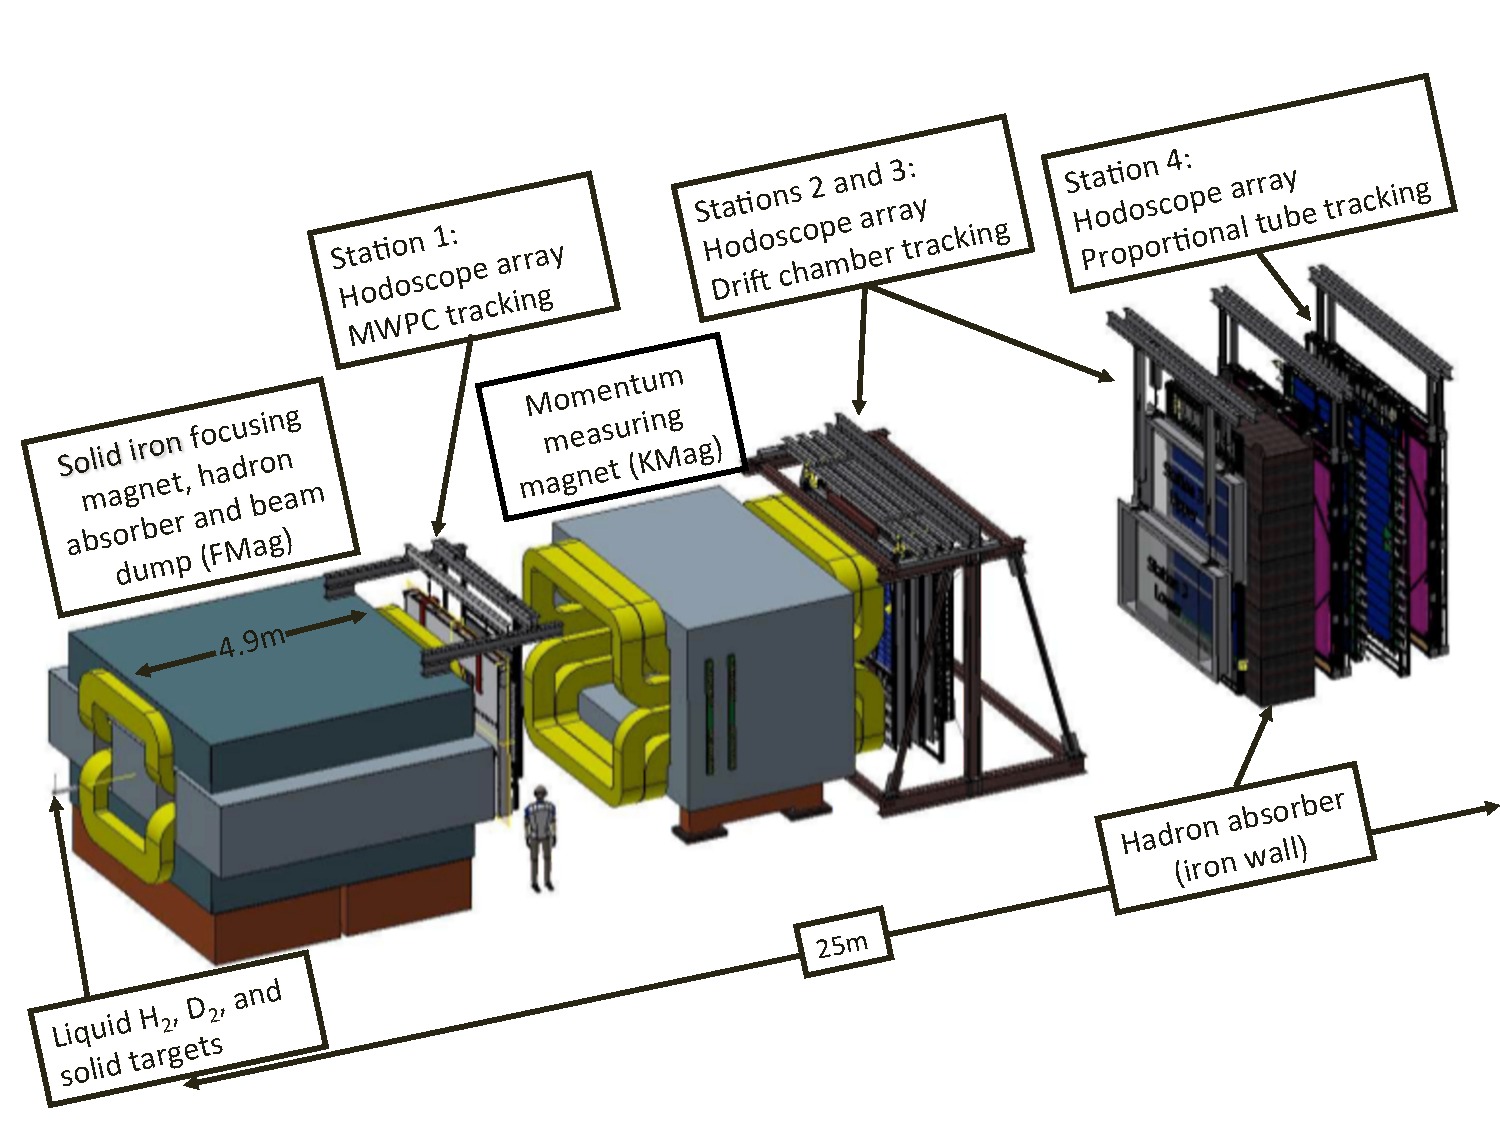
\includegraphics[width=0.6\linewidth]{SeaQuestSpectrometer}
	\caption{schematics of the SeaQuest spectrometer. Taken from Ref.~\cite{aidala2019}}
	\label{fig:spectrometer}
\end{figure}


\section{Beam}
\pdfmargincomment{A brief description of the beam structure, how the beam intensity
	is monitor. And finally says that the varying instantaneous beam intensity
	allows us to do intensity extrapolation which will be discussed in next
	chapter}
The layout of the Fermilab accelerator complex is shown in \cref{fig:complex}.
SeaQuest received its \SI{120}{\GeV} proton beam from the Fermilab Main Injector.
The proton beam originate from a direct-extraction magnetron hydrogen ion source,
which produce a \SI{35}{\keV} negative hydrogen ion beam. It is then accelerated
to \SI{750}{\keV} using Radio-frequency Quadrupole. Then the Linac accelerate the
$H^-$ ions to \SI{400}{\MeV}. The $H^-$ ions are then sent through a stripping foil
to remove the electrons. The resulting proton beam then circulates in the Booster
accelerator and accelerates to \SI{8}{\GeV}. The \SI{8}{\GeV} proton beam is
further accelerated by the Main Injector to \SI{120}{\GeV}. The proton beam is
extracted from the Main Injector using a process known as resonant extraction to
provide a lower intensity beam over a 5 second spill. The extracted beam, which
is sent to SeaQuest, retains the \SI{53.1}{\MHz} structure of the Main
Injector RF frequency, dividing the beam in to ``RF buckets'' that are less than
\SI{2}{\ns} long and occur every \SI{18.8}{\ns}.
\begin{figure}[htbp!]
	\centering
	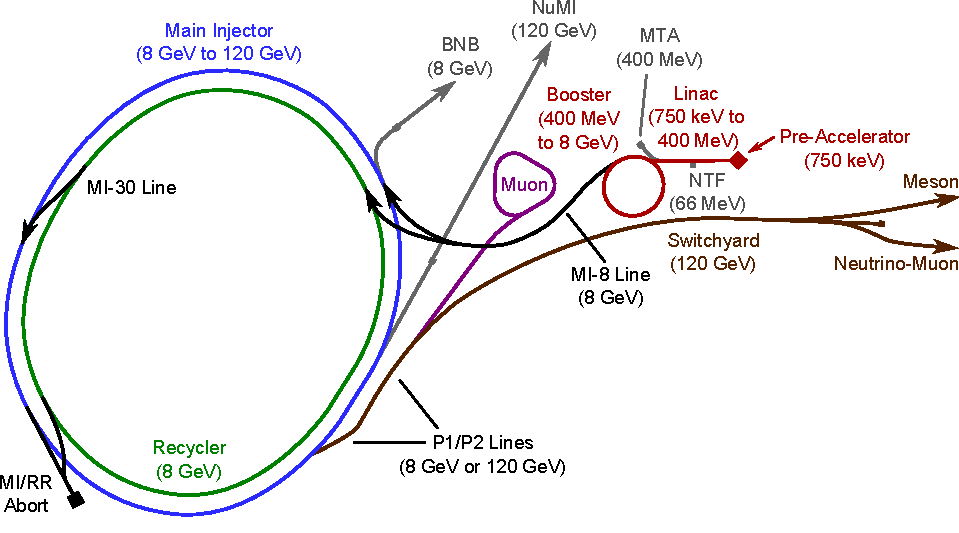
\includegraphics[width=0.6\linewidth]{Fermilab-complex}
	\caption{Layout of the Fermilab accelerator complex. Taken from Ref.~\cite{concept-book}}
	\label{fig:complex}
\end{figure}
However the number of protons in each bucket varies greatly during the spill, as
is shown in \cref{fig:intensity}.
\begin{figure}[htpb!]
	\centering
	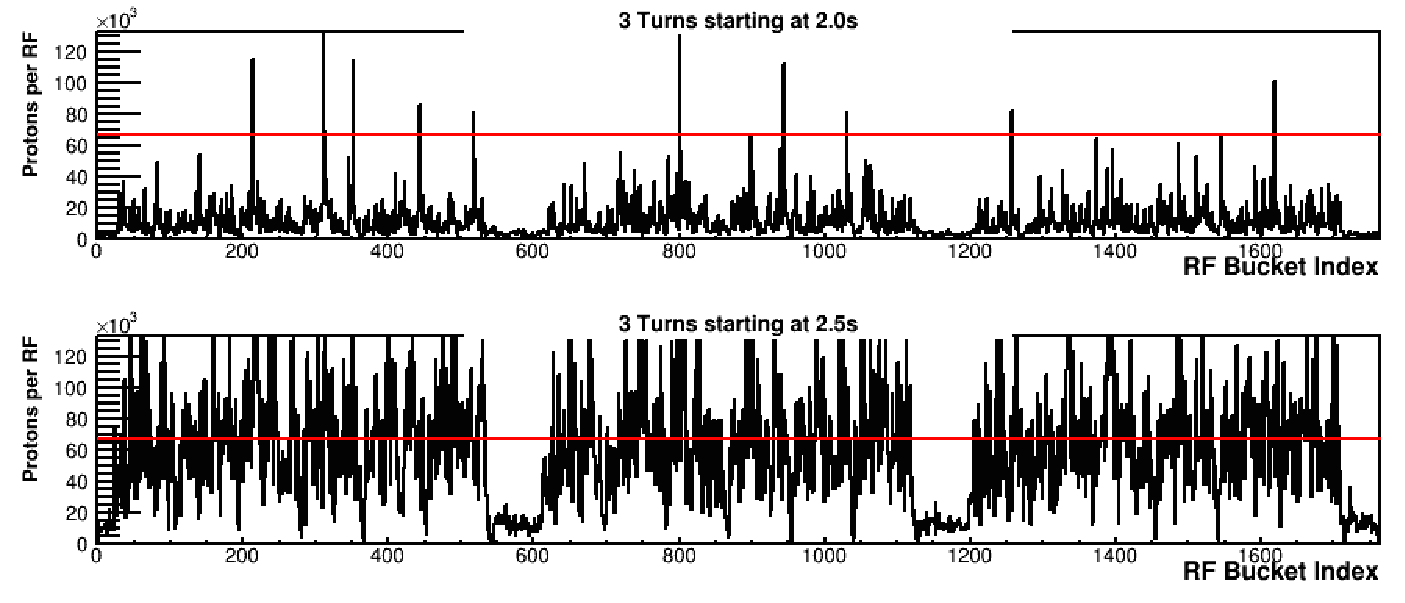
\includegraphics[width =0.8\linewidth]{beam_intensity_v2}
	\caption{The beam intensity measured by the Beam DAQ Cerenkov counter every
		bucket. Taken from Ref.~\cite{aidala2019}}
	\label{fig:intensity}
\end{figure}

\subsection{Beam Intensity Monitor}
The beam intensity is monitored using a Cerenkov counter, shown in \cref{fig:BIM}.
\begin{figure}[htbp!]
	\centering
	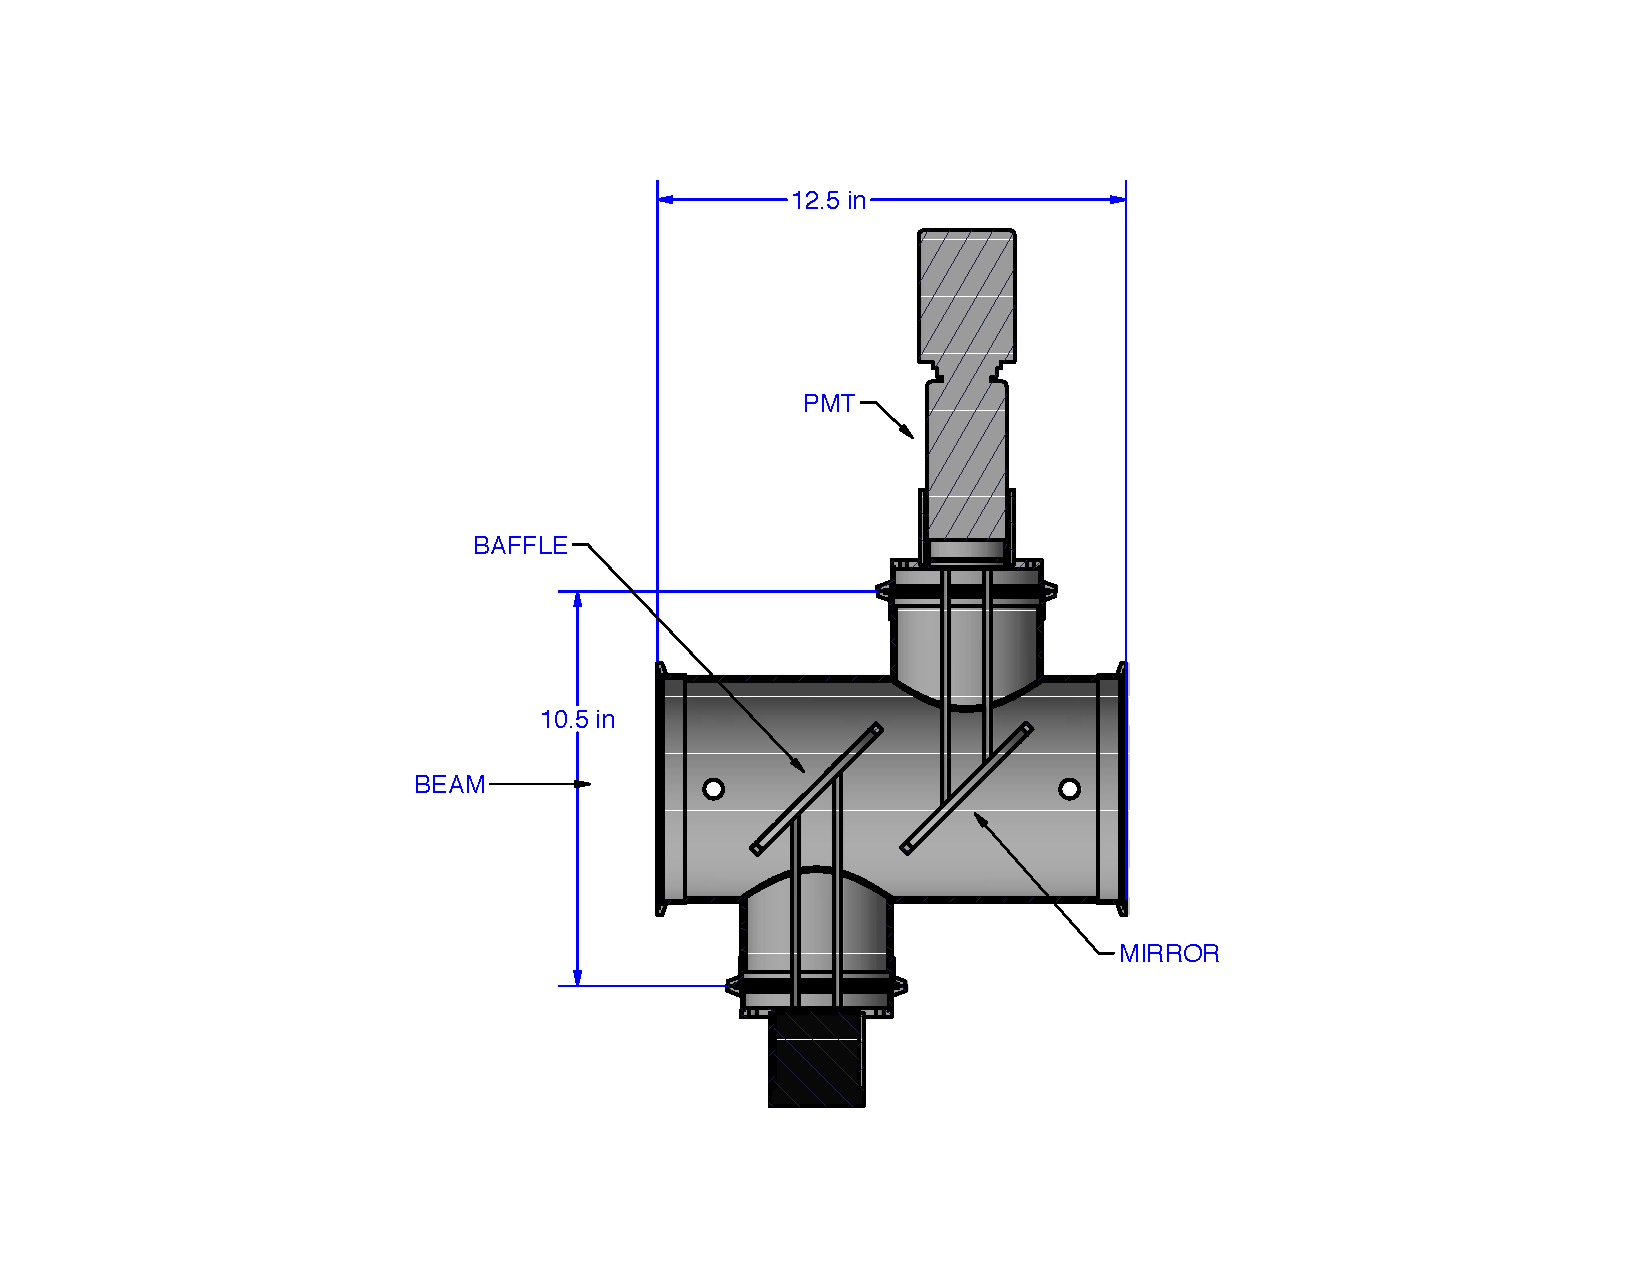
\includegraphics[width=0.4\linewidth]{BIMCerenkov}
	\caption{The Beam Intensity Monitor (BIM) Cerenkov counter. Taken from Ref.\
		\cite{aidala2019}.}
	\label{fig:BIM}
\end{figure}
A aluminized Kapton mirror reflect the Cerenkov light, produced when the proton beam
passing through the radiator, into a single photomultiplier tube. The signal is then
sent to a custom ``QIE'' (Charge Integrator and Encoder) module. This custom module
is clocked with the Main Injector RF, and is capable to recording the beam intensity
of each RF bucket for the entire spill. The QIE module is linked to the trigger
system, and would raise a trigger inhibit when the beam intensity is above a
threshold. The module is also read out by the Beam DAQ, which provides the (a)
integrated beam intensity for entire spill; (b) integrated beam while inhibit is
asserted at trigger logic; (c) integrated intensity during dead time; (d) a snapshot
of the beam intensity close in time to the trigger; and (e) a complete record of the
bucket-bucket intensity for the entire spill.

The ability to record the numbers of proton in each bucket allows us the obtain the
yield ratios as a function of the instantaneous intensity, which will be discussed
further in \cref{M-sec:extrapolation}


\section{Target}
\pdfmargincomment{list the properties of the targets. Some past thesis quoted the
	wrong number. Check PDG}
The SeaQuest target is placed between the Beam Intensity Monitor and the front face
of FMag. The target system consists of two liquid targets, hydrogen and deuterium,
and three solid targets, iron, carbon and tungsten. Each solid target is divided
into \num{3} discs of equal length, and are spatially separated along the beam
direction to minimize variation in acceptance between liquid and solid targets.
To account for background originating from the interaction with the instruments,
there are also two calibration targets, an empty vacuum filled flask, known as
empty flask, and the solid target holder, known as no-target. The different targets
are mounted on a motorized table, shown in \cref{fig:target}, which allows the
targets to be interchanged between spills to minimized systematic effect due to
spectrometer performance. The properties of the targets and the spills per cycle
of each target positions are listed in \cref{table:target}.
\pdfmargincomment{schematics of target system}
\begin{figure}[htbp!]
	\centering
	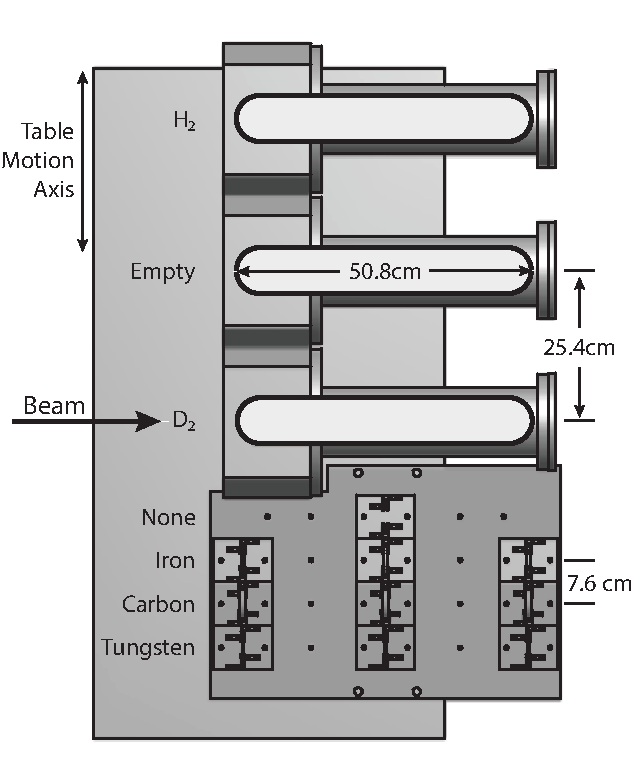
\includegraphics[width=0.4\linewidth]{target-tableLayout}
	\caption{The schematic of the movable target table}
	\label{fig:target}
\end{figure}

\begin{table}[h!]
	\centering
	\caption{SeaQuest target configuration}
	\label{table:target}
	\begin{tabular}{cccccc}
		\hline
		Target      & Position & Density (\unit{\g\per\cm\cubed}) & length (\unit{\cm}) & interaction length   (\unit{\g\per\cm\squared}) & spill/cycle \\ \hline
		\ce{LH_2}   & 1        & \num{0.071}                      & \num{50.8}          & \num{52.0}                                      & 10          \\
		Empty Flask & 2        & -                                & -                   & -                                               & 2           \\
		\ce{LD_2}   & 3        & \num{0.1634}                     & \num{50.8}          & \num{71.8}                                      & 5           \\
		No target   & 4        & -                                & -                   & -                                               & 2           \\
		Iron        & 5        & \num{7.87}                       & \num{1.905}         & \num{132.1}                                     & 1           \\
		Carbon      & 6        & \num{1.80}                       & \num{3.322}         & \num{85.8}                                      & 2           \\
		Tungsten    & 7        & \num{19.30}                      & \num{0.953}         & \num{191.9}                                     & 1           \\
	\end{tabular}
\end{table}

\section{Magnets}
There are two dipole magnets used in the SeaQuest spectrometer. The upstream magent (FMag)
is a solid iron magnet. The magent consists of a stack of high purity iron, recovered from
the Columbia University Nevis Laboratory Cyclotron, and the aluminium coils from the E866
SM3 magent. The coils are excited to \SI{2000}{\ampere} and generate a \SI{1.9}{\tesla}
magnetic field within the iron block. This correponds to a transverse momentum kick of
\SI{3.07}{\GeV}. FMag serves three main purpose: focuing high mass muon pairs, beam
dump and hadron absorber.

The downstream magent (KMag) is a \SI{3}{\meter} opeb aperture magnet. The coils are excited
to \SI{1600}{\ampere} which produce a magnetic field of \SI{0.4}{\tesla} correponding to a
\SI{0.41}{\GeV} transverse momentum kick. The primary purpose for KMag is to determine
the momentum of the muons.

\section{Tracking Station}
The SeaQuest detector system is separated into four tracking stations. Stations \num{1},
\num{2} and \num{3} comprise of hodoscopes and drift chambers. Whereas station \num{4}
comprises of hodoscope and proportional tubes. The hodoscopes in each stations provides
a fast signal for triggering whereas the drift chambers provide good spatial resolution
for precise reconstruction. The proportional tubes at station 4 is also used for muon
identification.

\subsection{Hodoscope}
The primary purpose of the scintillator hodoscopes are to provide fast singal for
trigger system. The x-palnes are placed vertically to measure the bend plane position.
And the y-planes are arranged horizontally to measure the non-bend plane position.

Station 1 and 2 each have single x-y planes. Station 3 ahs a single x plane, and station
4 has two y planes and one x plane. The scintillator bars used in St 1 and 2 are recycled
from HERMES experiment\pdfcomment{References}, whereas new Eljen EJ-200 scintillator material
is used for St 3 and 4. Because of the physical size of the sin bars in St4, the station 4
hodoscopes have PMTs on both ends of the sintillator bars. Each of the PMT base has a
``clip line'' attached at the output to reduce the output pulse from $20-25$\unit{\ns}
down to $10-15$\unit{\ns} full width.

The configuration of the hodoscope is summariezed in \cref{table:hodo}. \pdfmargincomment{why are there 2 y hodo in St4? Lower rate at St4? Shivangi's thesis is correct NIM paper is wrong}
\begin{table}[h!]
	\centering
	\caption{SeaQuest hodoscope configuration}
	\label{table:hodo}
	\begin{tabular}{lllllll}
		\hline
		Plane & Number      & Length (\unit{\cm}) & Width (\unit{\cm}) & Thickness (\unit{\cm}) & Array Width (\unit{\cm}) & Location (\unit{\cm})                                                 \\ \hline
		1Y    & $20\times2$ & \num{78.7}          & \num{7.32}         & \num{0.64}             & \num{140}                & \num{667}                                                             \\
		1X    & $23\times2$ & \num{69.9}          & \num{7.32}         & \num{0.64}             & \num{161}                & \num{654}                                                             \\
		2Y    & $19\times2$ & \num{132.0}         & \num{13.0}         & \num{0.64}             & \num{241}                & \num{1402}                                                            \\
		2X    & $16\times2$ & \num{152.0}         & \num{13.0}         & \num{0.64}             & \num{203}                & \num{1421}                                                            \\
		3X    & $16\times2$ & \num{167.6}         & \num{14.6}         & \num{1.3}              & \num{224}                & \num{1958}                                                            \\
		4Y1   & $16\times2$ & \num{152.4}         & \num{23.5}         & \num{1.3}              & \num{366}                & \begin{tabular}[c]{@{}l@{}}\num{2130}(L)\\ \num{2146}(R)\end{tabular} \\
		4Y2   & $16\times2$ & \num{152.4}         & \num{23.5}         & \num{1.3}              & \num{366}                & \begin{tabular}[c]{@{}l@{}}\num{2200}(L)\\ \num{2217}(R)\end{tabular} \\
		4X    & $16\times2$ & \num{182.9}         & \num{19.6}         & \num{1.3}              & \num{305}                & \begin{tabular}[c]{@{}l@{}}\num{2236}(T)\\ \num{2251}(B)\end{tabular} \\
	\end{tabular}
\end{table}

\subsection{Drift Chambers}
The primary purpose of the Drift Chambers is to provide better position resolution of the muons
at each station. Each drift chamber consist of six planes of sense wires. The wires in two planes,
denoted as x and x$'$, are aligned vertically. Two planes are tilted by \ang[retain-explicit-plus]{+14},
denoted as u and u$'$, and two planes are tilted by \ang[retain-explicit-plus]{-14}. The wires
in the primed planes are offset by half a drift cell to resolve left-right ambiguity of the
drift direction. Station 1 and 2 each have one chamber referred as D1 and D3. The chamber at station
3 is separated into top and bottom halve, D3p and D3m.

In data sets 1-3, a smaller chamber, D1.1, was used. It was latter replaced by a newly constructed
chamber, D1.2, with better expected high rate capacity in data set 4-6. However, D1.1 would be 
reinstalled later for data set 5-6. D3m.1 was used during the commissioning run, data set 1, and
was latter replaced by D3m.2 for the latter data sets.

The D1.1, D2 and D3m.1 chambers was recycled from previous Fermilab experiments, E605 (D2 and D3m.1)
and E866 (D1.1). The other chambers were designed and constructed for the SeaQuest experiment.
\pdfmargincomment{why do we have separate top and bottom chamber for D3 }
Specification of each chamber are listed in \cref{table:chamber}.

\begin{table}[h!]
	\centering
	\caption{SeaQuest drift chamber configuration. The primed planes are almost the same as the unprimed
		planes. The position of the x planes is defined to be the distance between the chamber and the
		upstream face of FMag, while the position for u and v denote the offset relative to the x plane.}
	\label{table:chamber}
	\begin{tabular}{cccccc}
		\hline
		Chamber & Plane & \# of wires & Cell width (\unit{\cm}) & Width\texttimes Height (\unit{\cm}\texttimes\unit{\cm}) & z Position (\unit{cm}) \\ \hline
		D1.1    & X     & \num{160}   & \num{0.64}              & $102\times 122$                                         & \num{617}              \\
		        & U, V  & \num{201}   & \num{0.64}              & $101\times 122$                                         & $\pm20$                \\
		D1.2    & X     & \num{320}   & \num{0.50}              & $153\times 137$                                         & \num{691}              \\
		        & U, V  & \num{384}   & \num{0.50}              & $153\times 137$                                         & $\pm1.2$               \\
		D2      & X     & \num{112}   & \num{2.1}               & $233\times264$                                          & \num{1347}             \\
		        & U, V  & \num{128}   & \num{2.0}               & $233\times264$                                          & $\pm25$                \\
		D3p     & X     & \num{116}   & \num{2.0}               & $232\times166$                                          & \num{1931}             \\
		        & U, V  & \num{134}   & \num{2.0}               & $268\times166$                                          & $\pm6$                 \\
		D3m.1   & X     & \num{176}   & \num{1.0}               & $179\times168$                                          & \num{1879}             \\
		        & U, V  & \num{208}   & \num{1.0}               & $171\times163$                                          & $\pm19$                \\
		D3m.2   & X     & \num{116}   & \num{2.0}               & $232\times166$                                          & \num{1895}             \\
		        & U, V  & \num{134}   & \num{2.0}               & $268\times166$                                          & $\pm6$
	\end{tabular}
\end{table}

\subsection{Proportional tubes}
The muon identification is accomplished with the proportional tube at station 4. A \SI{1}{\meter} thick
iron wall separate station 3 and 4, which act as an absorber to stop hadrons and electrons from reaching
station 4. For precise track reconstruction, there are four layers of proportional tubes planes. Each plane
is made up of eight proportional tube modules, with 16 proportional tubes per module. The 16 proportional tubes
in each module further divided into two sub-layers, with the second layers shifted by half a tube width to
resolve the left-right ambiguity, as in the case of drift chambers. The proportional tubes orientated horizontally
(vertically) are in the first and fourth (second and third) planes as shown in \cref{fig:prop}
The proportional tube modules were originally used in a Homeland Security project at Los Alamos National Laboratory.

\begin{figure}[ht!]
\centering
\begin{subfigure}{0.45\linewidth}
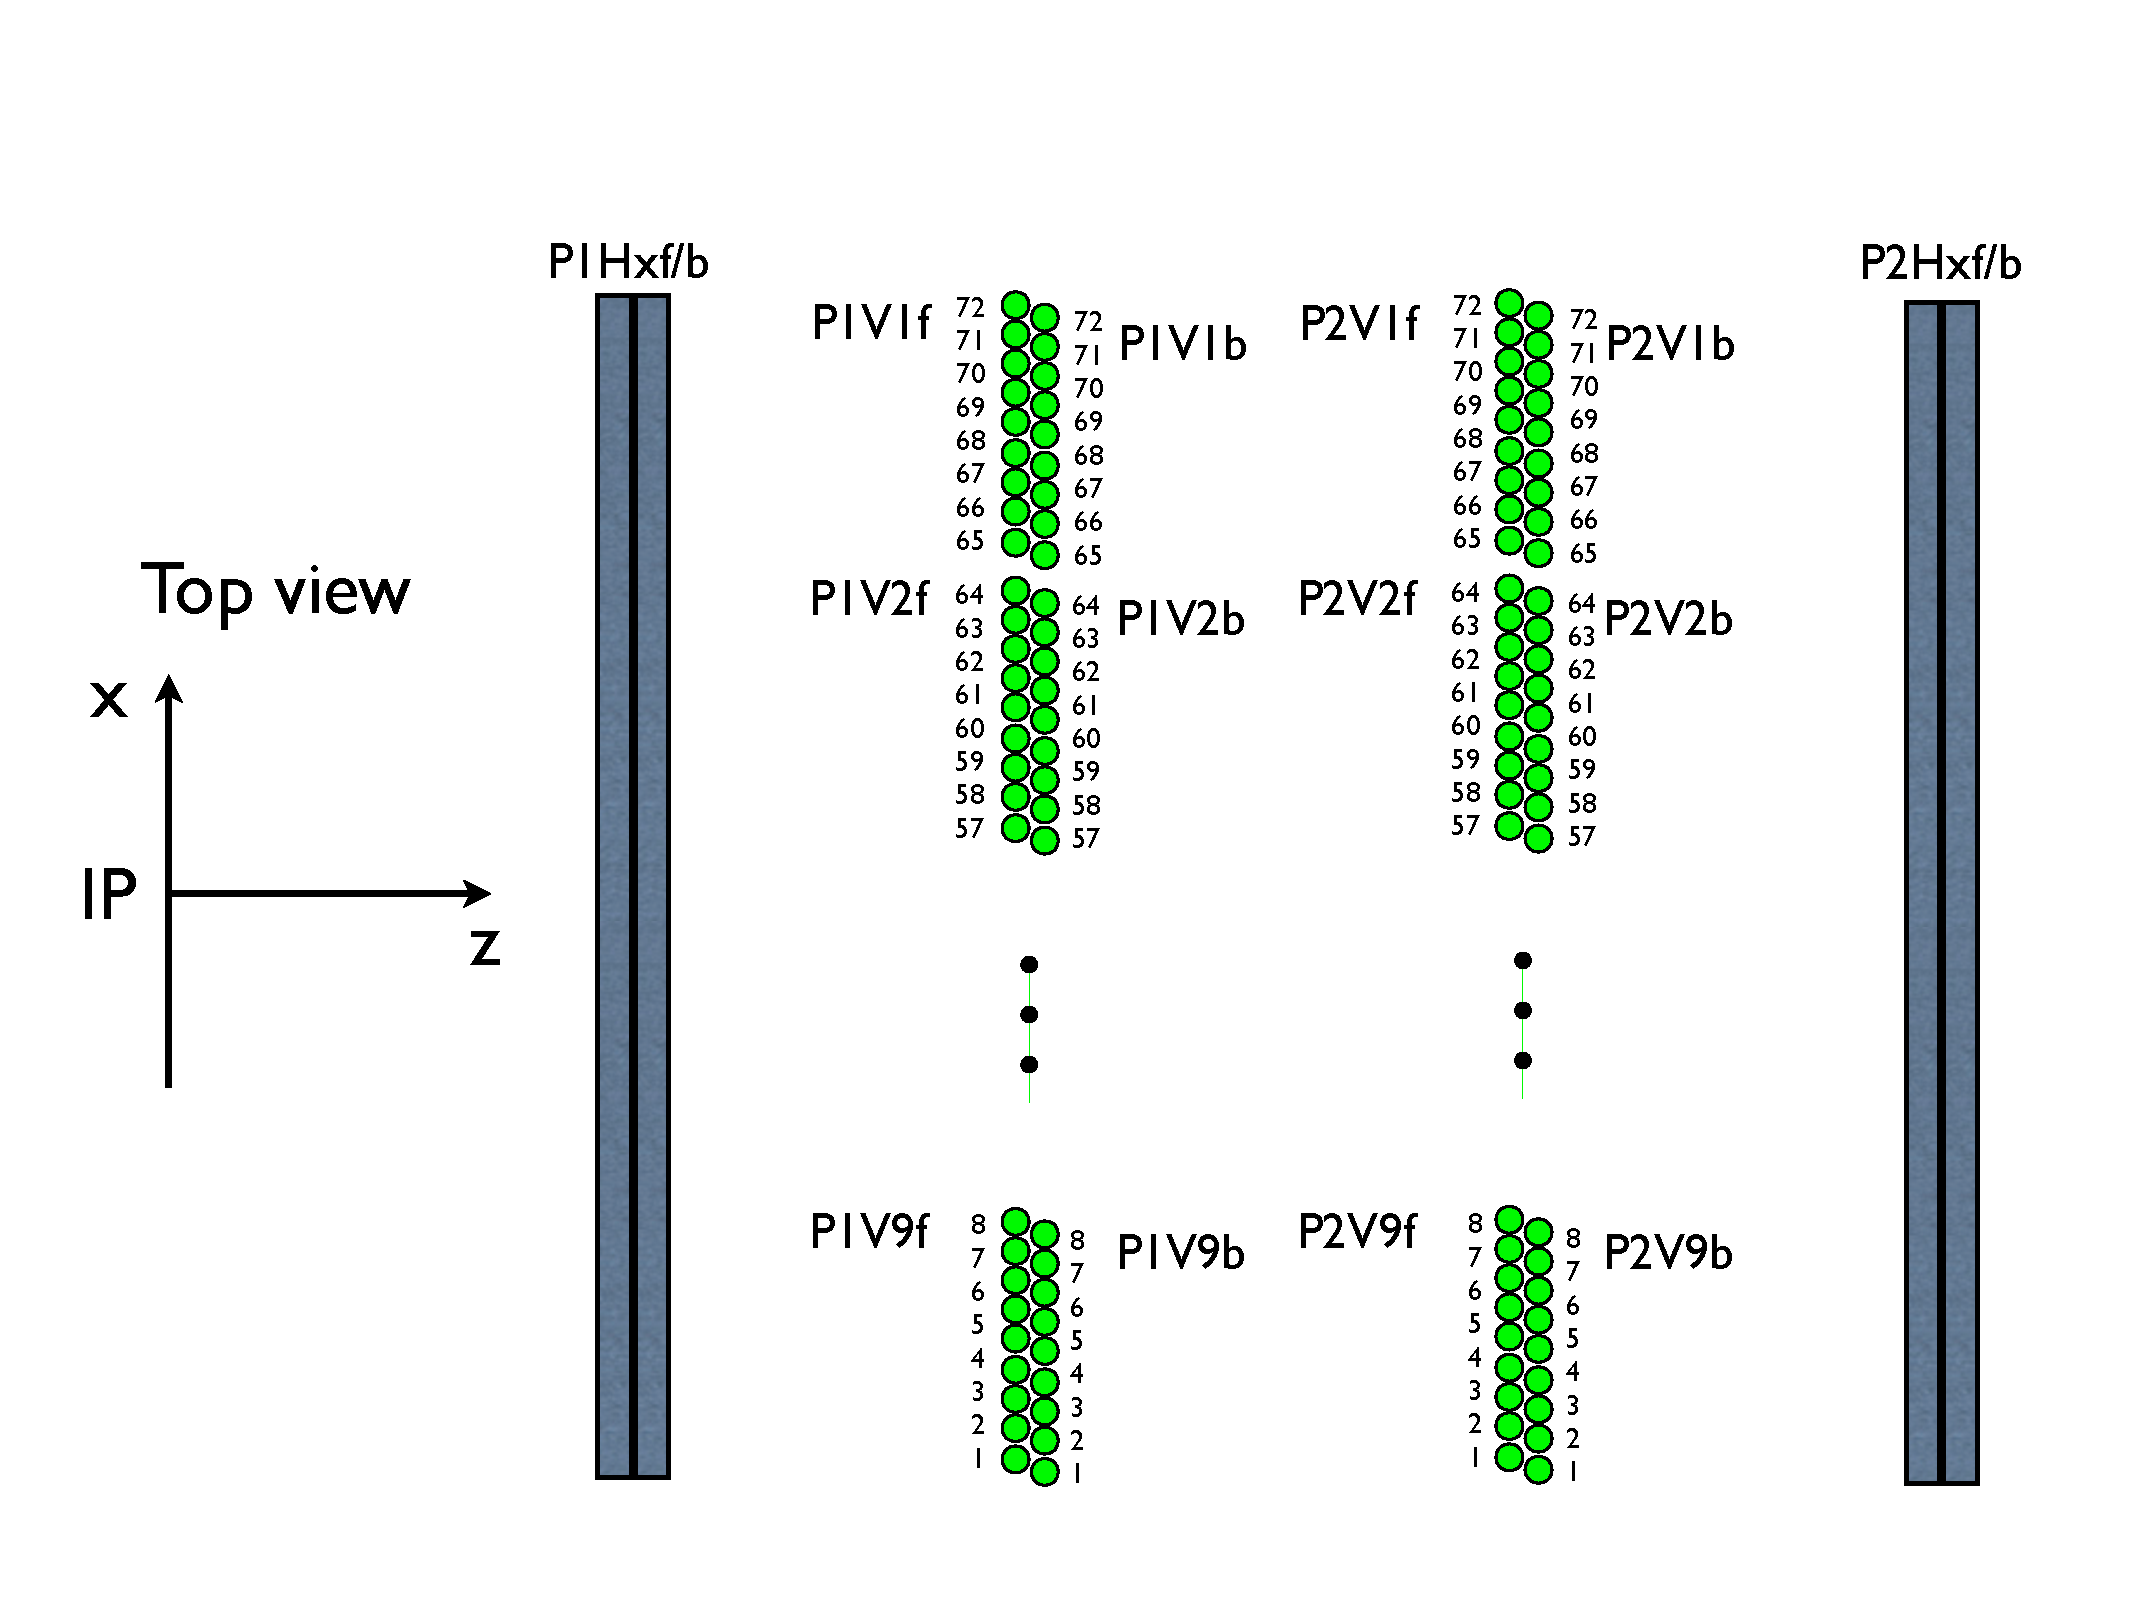
\includegraphics[width=0.9\linewidth]{proptubeview_xz}
\end{subfigure}
\begin{subfigure}{0.45\linewidth}
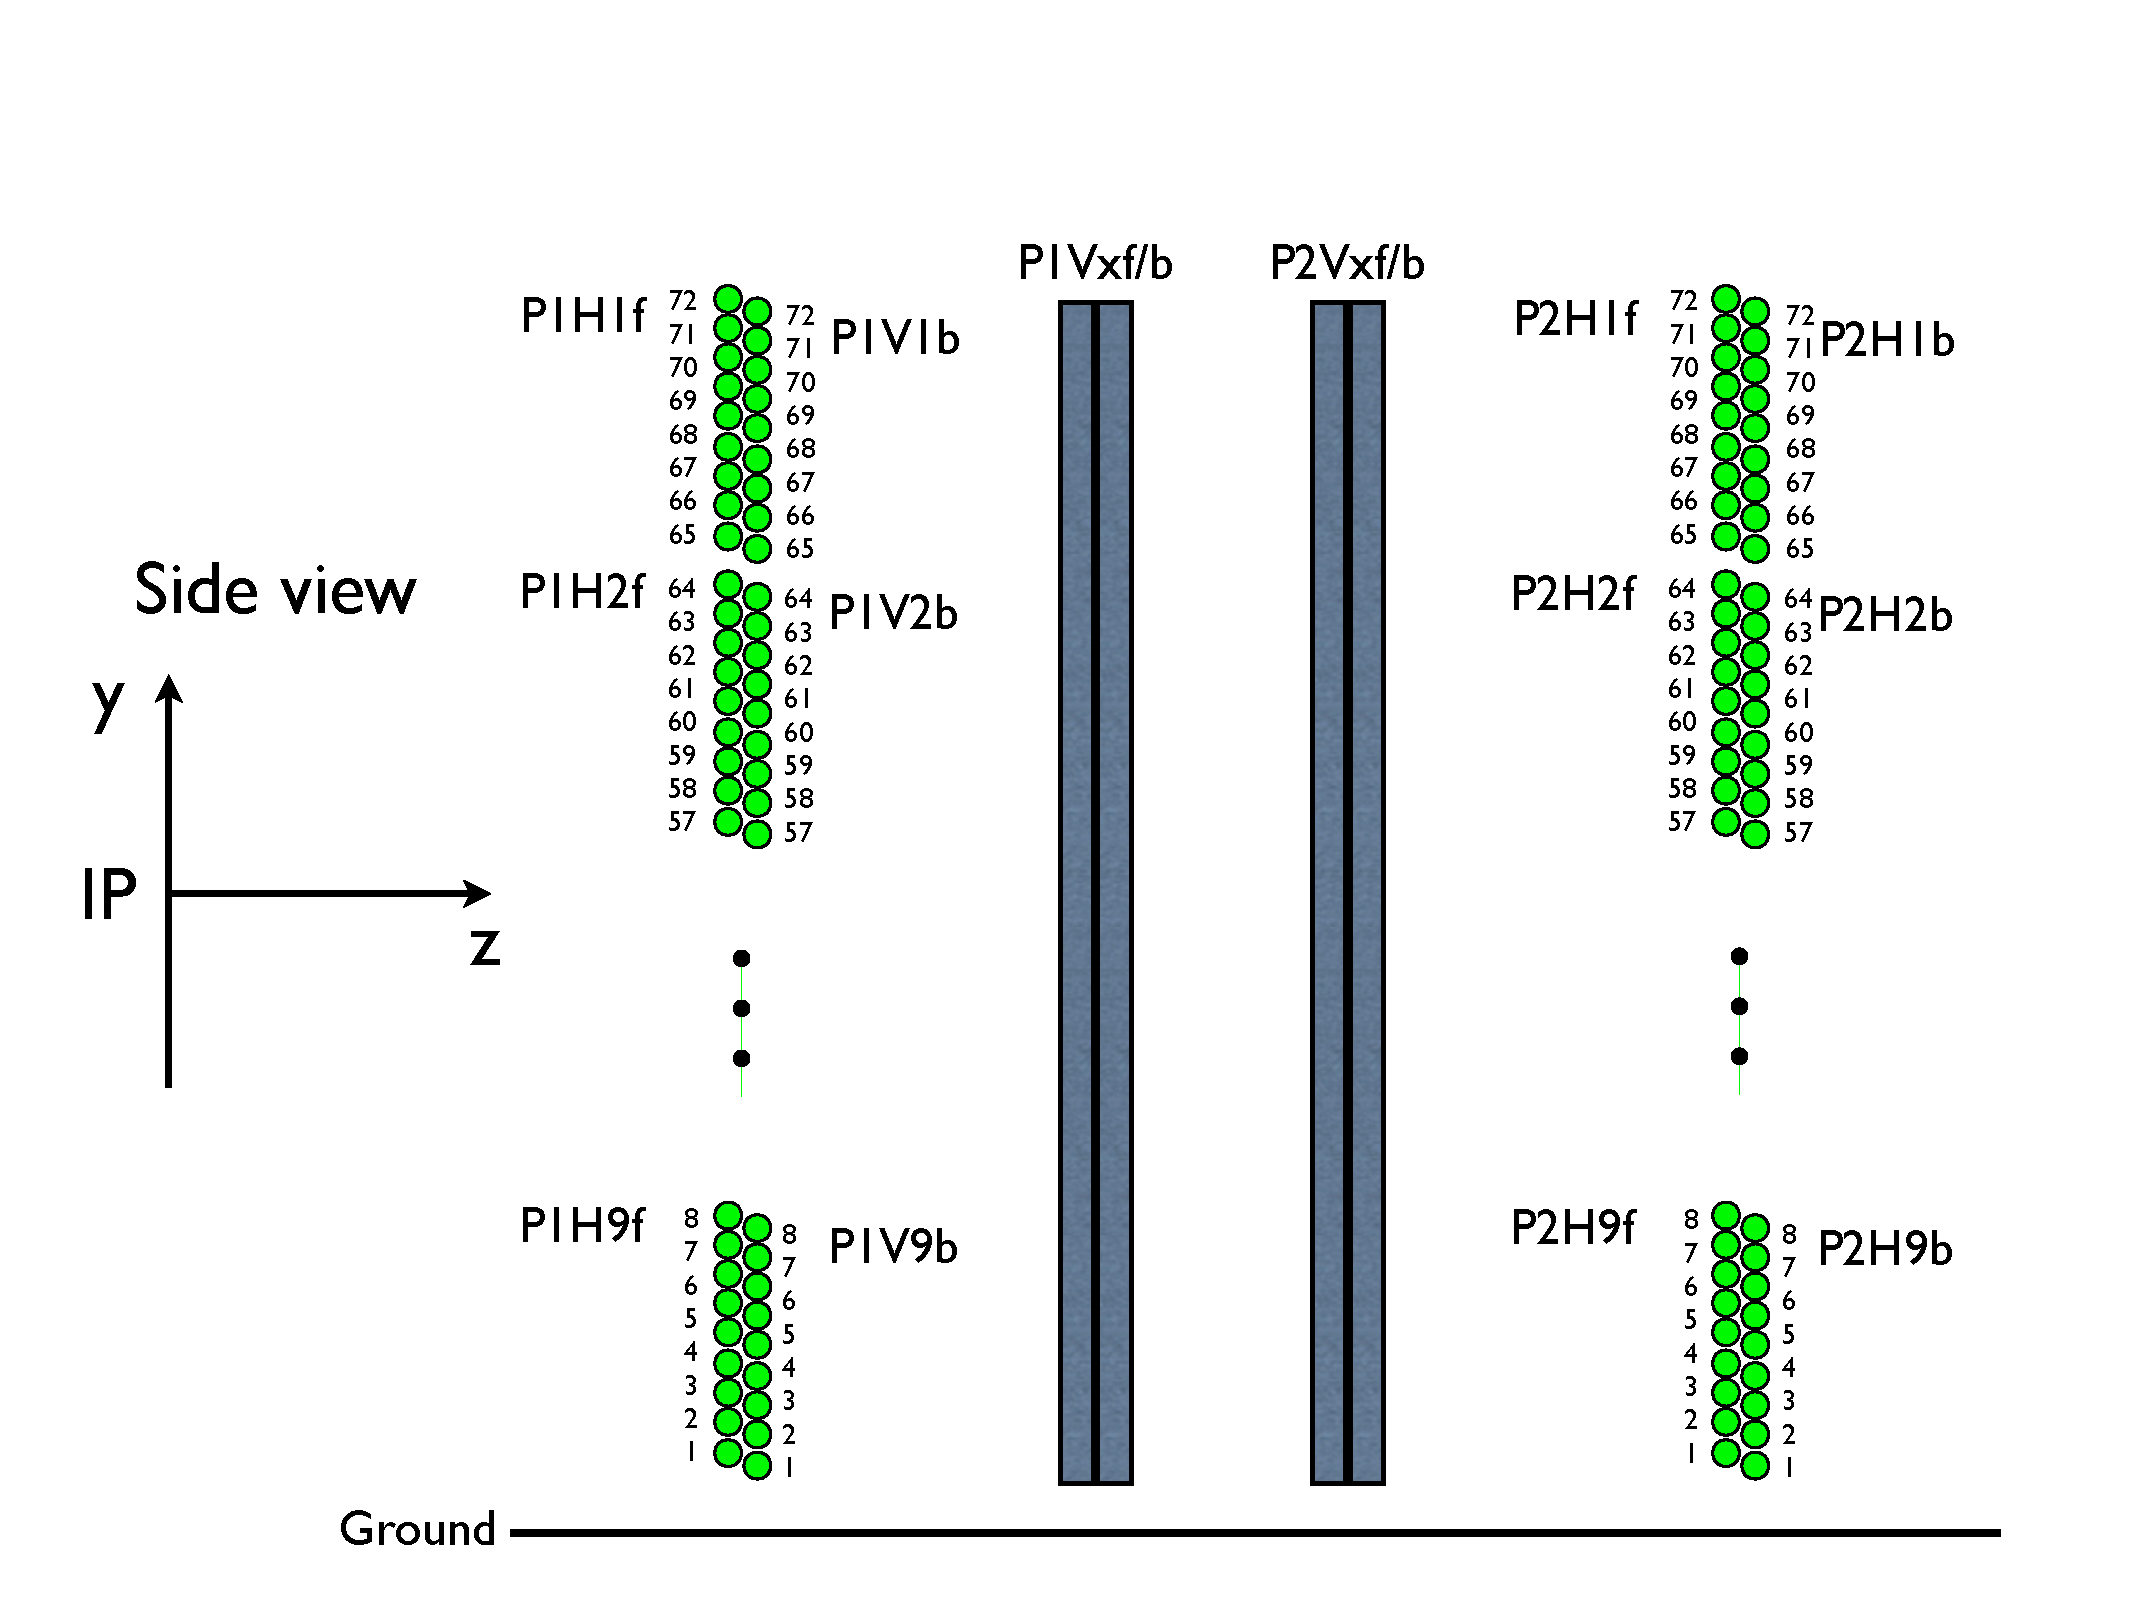
\includegraphics[width=0.9\linewidth]{proptubeview_yz}
\end{subfigure}
\caption{XZ (left) and YZ (left) view of the proportional tube at station 4.}
\label{fig:prop}
\end{figure}
\section{Trigger System}
The SeaQuest trigger uses discriminated signals from the hodoscope counters.
Two kinds of trigger systems are used in SeaQuest, NIM-based and FPGA-baesd.
The FPGA trigger system is the main trigger system. It utilizes uses 9 CAEN
v1495 VME modules, Altera EP1C20F400C6 FPGA (Field Programmable Gate Array)
modules. The 9 modules are separated into three levels from level 0 to level
2. Four FPGA modules form the level 0, with one module for each hodoscope
``quadrant'' (upper bend plane, lower bend plane, upper nonbend plane and
lower nonbend plane). During data taking, level 0 simply pass the input signal
to level 1. At level 1, four FPGA modules are used to search for four-hit track
candidates in each quadrant. The level 2 consists of a single module, and form
a trigger decision based on types of track candidates found at level 1. During
SeaQuest data taking, the are five output triggers, as listed in \cref{tab:FPGA}.
During SeaQuest, only x-measuring (bend plane) hodoscopes are used in making
trigger decisions.
\begin{table}[h!]
\centering
\caption{The five output trigger of the Level 2 trigger module.}
\label{tab:FPGA}
\begin{tabular}{lllll}
Name     & side  & Charge  & $p_x$ Req. & Notes                \\ \hline
Matrix 1 & TB/BT & $+-/-+$ & None       & Main physics trigger \\
Matrix 2 & TT/BB & $+-/-+$ & None       & Same-side trigger \\
Matrix 3 & TB/BT & $++/--$ & None       & Like-charge trigger \\
Matrix 4 & T/B & $+/-$ & None       & Single muon trigger \\
Matrix 5 & T/B & $+/-$ & $p_x>\SI{3}{\GeV}$       & High-$p_T$ single trigger                 
\end{tabular}
\end{table}


The NIM trigger utilizes Nuclear Instrumentation Modules to form the trigger
logic. During data taking, two types of NIM trigger are used, known as NIM-1
and NIM3. The NIM1 trigger is a coincidence of the y-measuring hodoscope hits
from all 4 stations. This trigger is mainly used for studying the efficiency
of the x-measuring hodoscope, which is important for understanding the performance
of the FPGA trigger system. The second NIM trigger, NIM-3 is also known as a
pulser trigger. It triggers on the coincidence of two clocks, a \SI{7.5}{\kHz}
clock generated by a gate generated by a gate generator and the \SI{53.1}{\MHz}
RF clock. The NIM-3 trigger is used to understand the intensity profile of the
beam and the background hits in the spectrometer. The hits from NIM-3 trigger
are also used in the Monte Carlo simulation to understand the rate dependence
of the reconstruction. This will be discussed further in \cref{M-sec:MC}.
\pdfmargincomment{the charge is determined from the px kick}


\ifSubfilesClassLoaded{ \printbibliography[heading=bibintoc,title={References}]}{}
\end{document}
